	%!TEX program = xelatex
% 完整编译: xelatex -> bibtex -> xelatex -> xelatex
\documentclass[lang=cn,12pt,a4paper,cite=authoryear]{elegantpaper}

\title{统计学习实验三:Logistics Regression}
\author{王嗣萱 2018110601014}
\date{}


% 本文档命令
\usepackage{array}
\newcommand{\ccr}[1]{\makecell{{\color{#1}\rule{1cm}{1cm}}}}

\begin{document}

\maketitle

\section{实验原理}

\subsection{Logistic 分布}
Logistic 分布是一种连续型的概率分布,其分布函数和密度函数分别为:
\begin{equation}
	\begin{aligned}
		&F(x) = P(X \leq x)=\frac{1}{1+e^{-(x-\mu)/\gamma}} \\
		&f(x) = 	F^{'}(X \leq x)=\frac{e^{-(x-\mu)/\gamma}}{\gamma(1+e^{-(x-\mu)/\gamma})^{2}}
	\end{aligned}
\end{equation}

其中, $\mu$ 表示位置参数, $\gamma$ 为形状参数。我们可以看下其图像特征:

\begin{figure}[htbp]
	\centering
	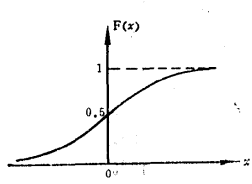
\includegraphics[width=0.3\textwidth]{lo_1.png}
	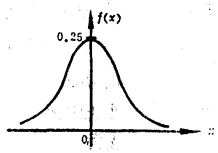
\includegraphics[width=0.3\textwidth]{lo_2.png}
	\caption{Logistic 分布}
\end{figure}

Logistic 分布是由其位置和尺度参数定义的连续分布。Logistic 分布的形状与正态分布的形状相似,但是 Logistic 分布的尾部更长,所以我们可以使用 Logistic 分布来建模比正态分布具有更长尾部和更高波峰的数据分布。在深度学习中常用到的 Sigmoid 函数就是 Logistic 的分布函数在  $\mu=0, \gamma=1$ 的特殊形式。

\subsection{Logistic 回归}
本次实验中考虑'0','1'的二分类问题,即一个伯努利分布。

Sigmoid函数,也称为逻辑函数(Logistic function):
\begin{equation}
	g(z)= \frac{1}{1+e^{-z}}
\end{equation}


逻辑回归的假设函数形式如下:
\begin{equation}
	\begin{aligned}
		&h_\theta(x) = g(\theta^T x), g(z)= \frac{1}{1+e^{-z}}
		\\
		&P(y=1|x;\theta)=h_{\theta}(x) 
		\\
		&P(y=0|x;\theta)=1-h_{\theta}(x)
	\end{aligned}
\end{equation}
可以将其合并为一个表达式:
\begin{equation}
	\begin{aligned}
		&P(y|x;\theta)=(h_{\theta}(x))^{y}(1-h_{\theta}(x))^{1-y}
	\end{aligned}
\end{equation}

logistic regression的目标函数是根据最大似然思想求得的。似然函数为:
\begin{equation}
	\begin{aligned}
		&L(\theta)=\prod_{i=1}^{n}(h_{\theta}(x^{i}))^{y^{i}}(1-h_{\theta}(x^{i}))^{1-y^{i}}
	\end{aligned}
\end{equation}


对$L(\theta)$求对数可以得到:
\begin{equation}
	\begin{aligned}
		&l(\theta)=-logL(\theta)=-\sum_{i=1}^{n}[{y^{i}}log(h_{\theta}(x^{i}))+(1-y^{i})log(1-h_{\theta}(x^{i}))]
	\end{aligned}
\end{equation}

使用$J(\theta)=\frac{1}{m}l(\theta)=-\frac{1}{N}logL(w) $作为logistic regression的损失函数


\subsection{梯度下降}

\begin{figure}[htbp]
	\centering
	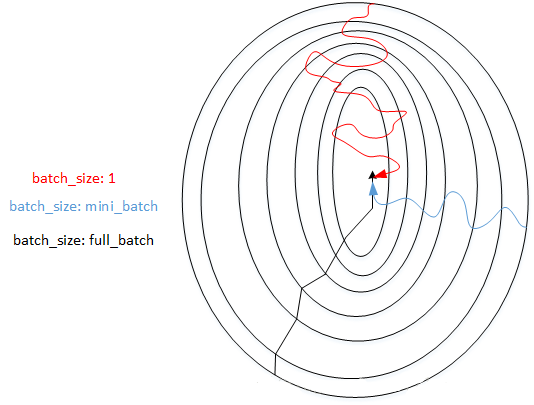
\includegraphics[width=0.3\textwidth]{batch.png}
	\caption{梯度下降}
\end{figure}

批量梯度下降每次迭代时使用所有样本进行梯度的更新,每次更新的梯度就是所有的梯度和,故当目标函数为凸函数时,一定可以达到全局最优,但是由于每次需要使用所有样本,因此训练过程非常慢,并且当样本非常大时将耗费巨大的计算资源和时间。


随机梯度下降每次迭代随机使用一个样本,因此每轮迭代将非常快,但是由于单个样本不能代表全局样本的趋势,故可能无法收敛,同时使最优解的准确度下降,但由于其速度上有非常好的优势,故现在大多数样本较大的机器学习采用该策略。随机梯度下降通常来说使得参数在大体上趋向于最优的,通常会达到最优解附近。


mini-batch梯度下降则是上述两种方法的折中,每次迭代采用batch-size个样本数据来对参数进行更新,故在该方法中size的选择通常是较为重要的,选择较好的size可以发挥批量梯度下降和随机梯度下降的优势,在较快的速度内完成迭代且最终有着不错的收敛效果。实际上当size选择为1的时候就是随机梯度下降,当size为data-size的时候则为批量梯度下降。


\section{Python代码实现}

\begin{lstlisting}
	import time
	import numpy as np
	import matplotlib.pyplot as plt
	import gzip as gz
	
	x_dim = 28 * 28
	y_dim = 2
	W_dim = (y_dim, x_dim)
	b_dim = y_dim
	
	alpha = 1e-6
	batch_size = 5  # 5,17,85,745,12665
	epochs_num = 1
	
	
	def load_data(filename, kind):
		with gz.open(filename, 'rb') as fo:
		buf = fo.read()
		index = 0
		if kind == 'data':
		header = np.frombuffer(buf, '>i', 4, index)
		index += header.size * header.itemsize
		data = np.frombuffer(buf, '>B', header[1] * header[2] * header[3], index).reshape(header[1], -1)
		elif kind == 'lable':
		header = np.frombuffer(buf, '>i', 2, 0)
		index += header.size * header.itemsize
		data = np.frombuffer(buf, '>B', header[1], index)
		return data
	
	
	def init_data():
		X_train = load_data('train-images-idx3-ubyte.gz', 'data')
		y_train = load_data('train-labels-idx1-ubyte.gz', 'lable')
		X_test = load_data('t10k-images-idx3-ubyte.gz', 'data')
		y_test = load_data('t10k-labels-idx1-ubyte.gz', 'lable')
		X_train = np.array(X_train[y_train <= 1, :])
		y_train = np.array(y_train[y_train <= 1])
		X_test = np.array(X_test[y_test <= 1, :])
		y_test = np.array(y_test[y_test <= 1])
		return X_train, y_train, X_test, y_test
	
	
	def softmax(x):
		return np.exp(x) / np.exp(x).sum()
	
	
	def loss(W, b, x, y):
		return -np.log(softmax(np.dot(W, x) + b)[y])  # 预测值与标签相同的概率
	
	
	def L_Gra(W, b, x, y):
		W_G = np.zeros(W.shape)
		b_G = np.zeros(b.shape)
		S = softmax(np.dot(W, x) + b)
		W_row = W.shape[0]
		W_column = W.shape[1]
		b_column = b.shape[0]
		for i in range(W_row):
		for j in range(W_column):
		W_G[i][j] = (S[i] - 1) * x[j] if y == i else S[i] * x[j]
		for i in range(b_column):
		b_G[i] = S[i] - 1 if y == i else S[i]
		return W_G, b_G
	
	
	def test_accurate(W, b, X_test, y_test):
		num = len(X_test)
		results = []
		for i in range(num):
		y_i = np.dot(W, X_test[i]) + b
		res = 1 if softmax(y_i).argmax() == y_test[i] else 0
		results.append(res)
		accurate_rate = np.mean(results)
		return accurate_rate
	
	
	def mini_batch(batch_size, alpha, epoches, X_train, y_train, X_test, y_test):
		accurate_rates = []
		W = np.zeros(W_dim)
		b = np.zeros(b_dim)
		x_batches = np.zeros(((int(X_train.shape[0] / batch_size), batch_size, 784)))
		y_batches = np.zeros(((int(X_train.shape[0] / batch_size), batch_size)))
		batches_num = int(X_train.shape[0] / batch_size)
		for i in range(0, X_train.shape[0], batch_size):
		x_batches[int(i / batch_size)] = X_train[i:i + batch_size]
		y_batches[int(i / batch_size)] = y_train[i:i + batch_size]
		print('Start training...')
		start = time.time()
		for epoch in range(epoches):
		for i in range(batches_num):
		W_gradients = np.zeros(W_dim)
		b_gradients = np.zeros(b_dim)
		x_batch, y_batch = x_batches[i], y_batches[i]
		for j in range(batch_size):
		W_g, b_g = L_Gra(W, b, x_batch[j], y_batch[j])
		W_gradients += W_g
		b_gradients += b_g
		W_gradients /= batch_size
		b_gradients /= batch_size
		W -= alpha * W_gradients
		b -= alpha * b_gradients
		accurate_rates.append(test_accurate(W, b, X_test, y_test))
		end = time.time()
		time_cost = (end - start)
		return W, b, time_cost, accurate_rates
	
	
	def run(alpha, batch_size, epochs_num, X_train, y_train, X_test, y_test):
		W, b, time_cost, accuracys = mini_batch(batch_size, alpha, epochs_num, X_train, y_train, X_test, y_test)
		print("Result: accuracy:{:.2%},time cost:{:.2f}".format(accuracys[-1], time_cost))
			plt.title('Model accuracy')
			plt.xlabel('Iterations')
			plt.ylabel('Accuracy')
			plt.plot(accuracys, 'm')
			plt.grid()
			plt.show()
			
			
	if __name__ == '__main__':
		X_train, y_train, X_test, y_test = init_data()
		run(alpha, batch_size, epochs_num, X_train, y_train, X_test, y_test)
		
\end{lstlisting}
\section{结果及图形展示}
\begin{figure}[htbp]
	\centering
	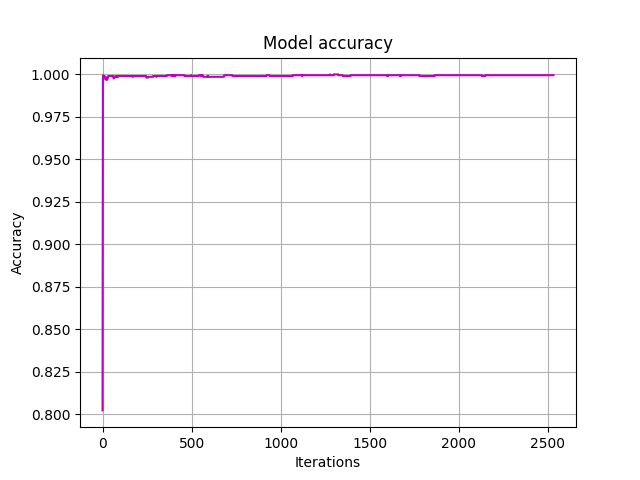
\includegraphics[width=0.5\textwidth]{accuracy.png}
	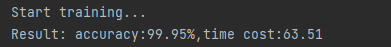
\includegraphics[width=0.5\textwidth]{cmd_1.png}
	\caption{batch size = 5}
\end{figure}
由于“1”“0”的差距很大,分类的准确率在前几次就已经达到了需求。
\begin{figure}[htbp]
	\centering
	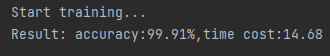
\includegraphics[width=0.5\textwidth]{cmd_3.png}
	\caption{batch size = 85}
\end{figure}
\begin{figure}[htbp]
	\centering
	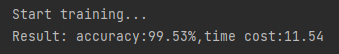
\includegraphics[width=0.5\textwidth]{cmd_2.png}
	\caption{批量梯度下降}
\end{figure}

使用的小批量梯度下降和批量梯度下降,对于该二分类问题,二者准确率都足够高。
\section{总结体会}
通过这次实验,了解了逻辑回归在分类上的作用和成效,其中又对于梯度下降中的小批量梯度下降法(MBGD)有了进一步的了解,虽然对于这个二分类问题中,由于分成的样本过多导致运行时间过长,但当样本更大时(扩展到十分类问题)MBGD的效率就会更高。
\end{document}
